\documentclass{article}
\usepackage{../../settings}

\begin{document}
\hexcover{Py 心寫程式}{學習歷程}{作者:曾嘉禾}{Dandelion}{電算社}

\begin{large}
\begin{boxpar}{Dandelion}{說明}
透過 Python 的 pygame 函式庫寫出一款圖形化介面的遊戲。
\end{boxpar}
\begin{boxpar}{Dandelion}{動機}
「除了在終端機上無聊的輸入輸出外,人們是怎麼樣利用程式語言寫出一款遊戲的呢?包括基本的視窗、按鈕、
    元件等等的圖形化介面元件是如何以程式處理的?」這個問題雖然已經在我的腦內迴盪了無數次,仍舊因為
    擔心自己實力不足而退卻不敢親身嘗試。直到後來來到了校內社團博覽會的電算社展區,看到他們是怎麼利用
    我已經學會的程式語言 python 寫出一款有趣的遊戲。所幸入社後社內學長姊慧眼獨具,任命我擔任靜態展
    學術長的要職。所以為了完成自己的職責以及解開一直以來對程式語言的疑惑,我選擇以 pygame 函式庫與
    組員一起撰寫一款遊戲。
\end{boxpar}
    \begin{boxpar}{Dandelion}{學習過程}
        在學習之前,找到對的方向是身為學習者最重要的步驟。一開始雖然已經選擇了 pygame 作為遊戲引擎,
        不過我因為擔心難度太高而搖擺在眾多的遊戲引擎之間搖擺。不過後來經過學長的勸導,發現要成功應該要抓著機會不迷惘的往前衝。所以後來靜下心來認真學習
        pygame 後發現沒有自己所想像中的難,讓自己重拾自己的信心完成這項重大的任務。
    \end{boxpar}
\begin{boxpar}{Dandelion}{遇到的問題:惱人的 pygame.display}
一開始常常遇到的問題就是 pyagme.display 的管理。之所以 GUI
    如此注重圖形處理,所以管理顯示器的 pygame.display
    就在遊戲內扮演重大的角色。不過在最初因為對它的不熟悉常常在執行程式時發生圖形錯位,令我頭痛不已。
    \begin{boxpar}{Dandelion}{解決方式}
        查詢 Documentation 是最簡單的解決方式。身為未來想當程式設計師的我,必須要學習如何閱讀
        Documentation。因為有時在問別人問題或放棄之前,其實可能有人在網路上早就解答過了。當時我有去
        \href{https://www.pygame.org/docs/ref/display.html}{pygame 官網} 查詢,更是
        \href{https://www.youtube.com/watch?v=C8YtdC8mxTU}{上 YouTube 取得幫助}。
        最後發現自己能夠以 pygame 表示 GUI 基礎元件,並且了解其中的原理,算是解答了一開始問題的一半了。
    \end{boxpar}
\end{boxpar}
\begin{boxpar}{Dandelion}{遇到的問題:組員之間無法溝通}
    作為一位領導者,團隊成員之間的溝通和任務分配至關重要。一開始由於溝通不足而誤解了團隊成員並認為
    他們在逃避工作。然而我為了解決這個問題召開一次次的線上會議,並且嘗試釐清每位成員的個別需求。
    這不但冰釋之前彼此之間的誤解,還讓我和團隊成員逐漸建立了良好的合作關係,融洽的一起完成手上的工作。
\end{boxpar}
\newpage
\begin{boxpar}{Dandelion}{成品}
    我把原始碼\href{https://github.com/hsnucrc46/crcproject}{commit 到 GitHub
    上}並且以 GPLv3 的 copyleft 授權書授權。
    圖片
    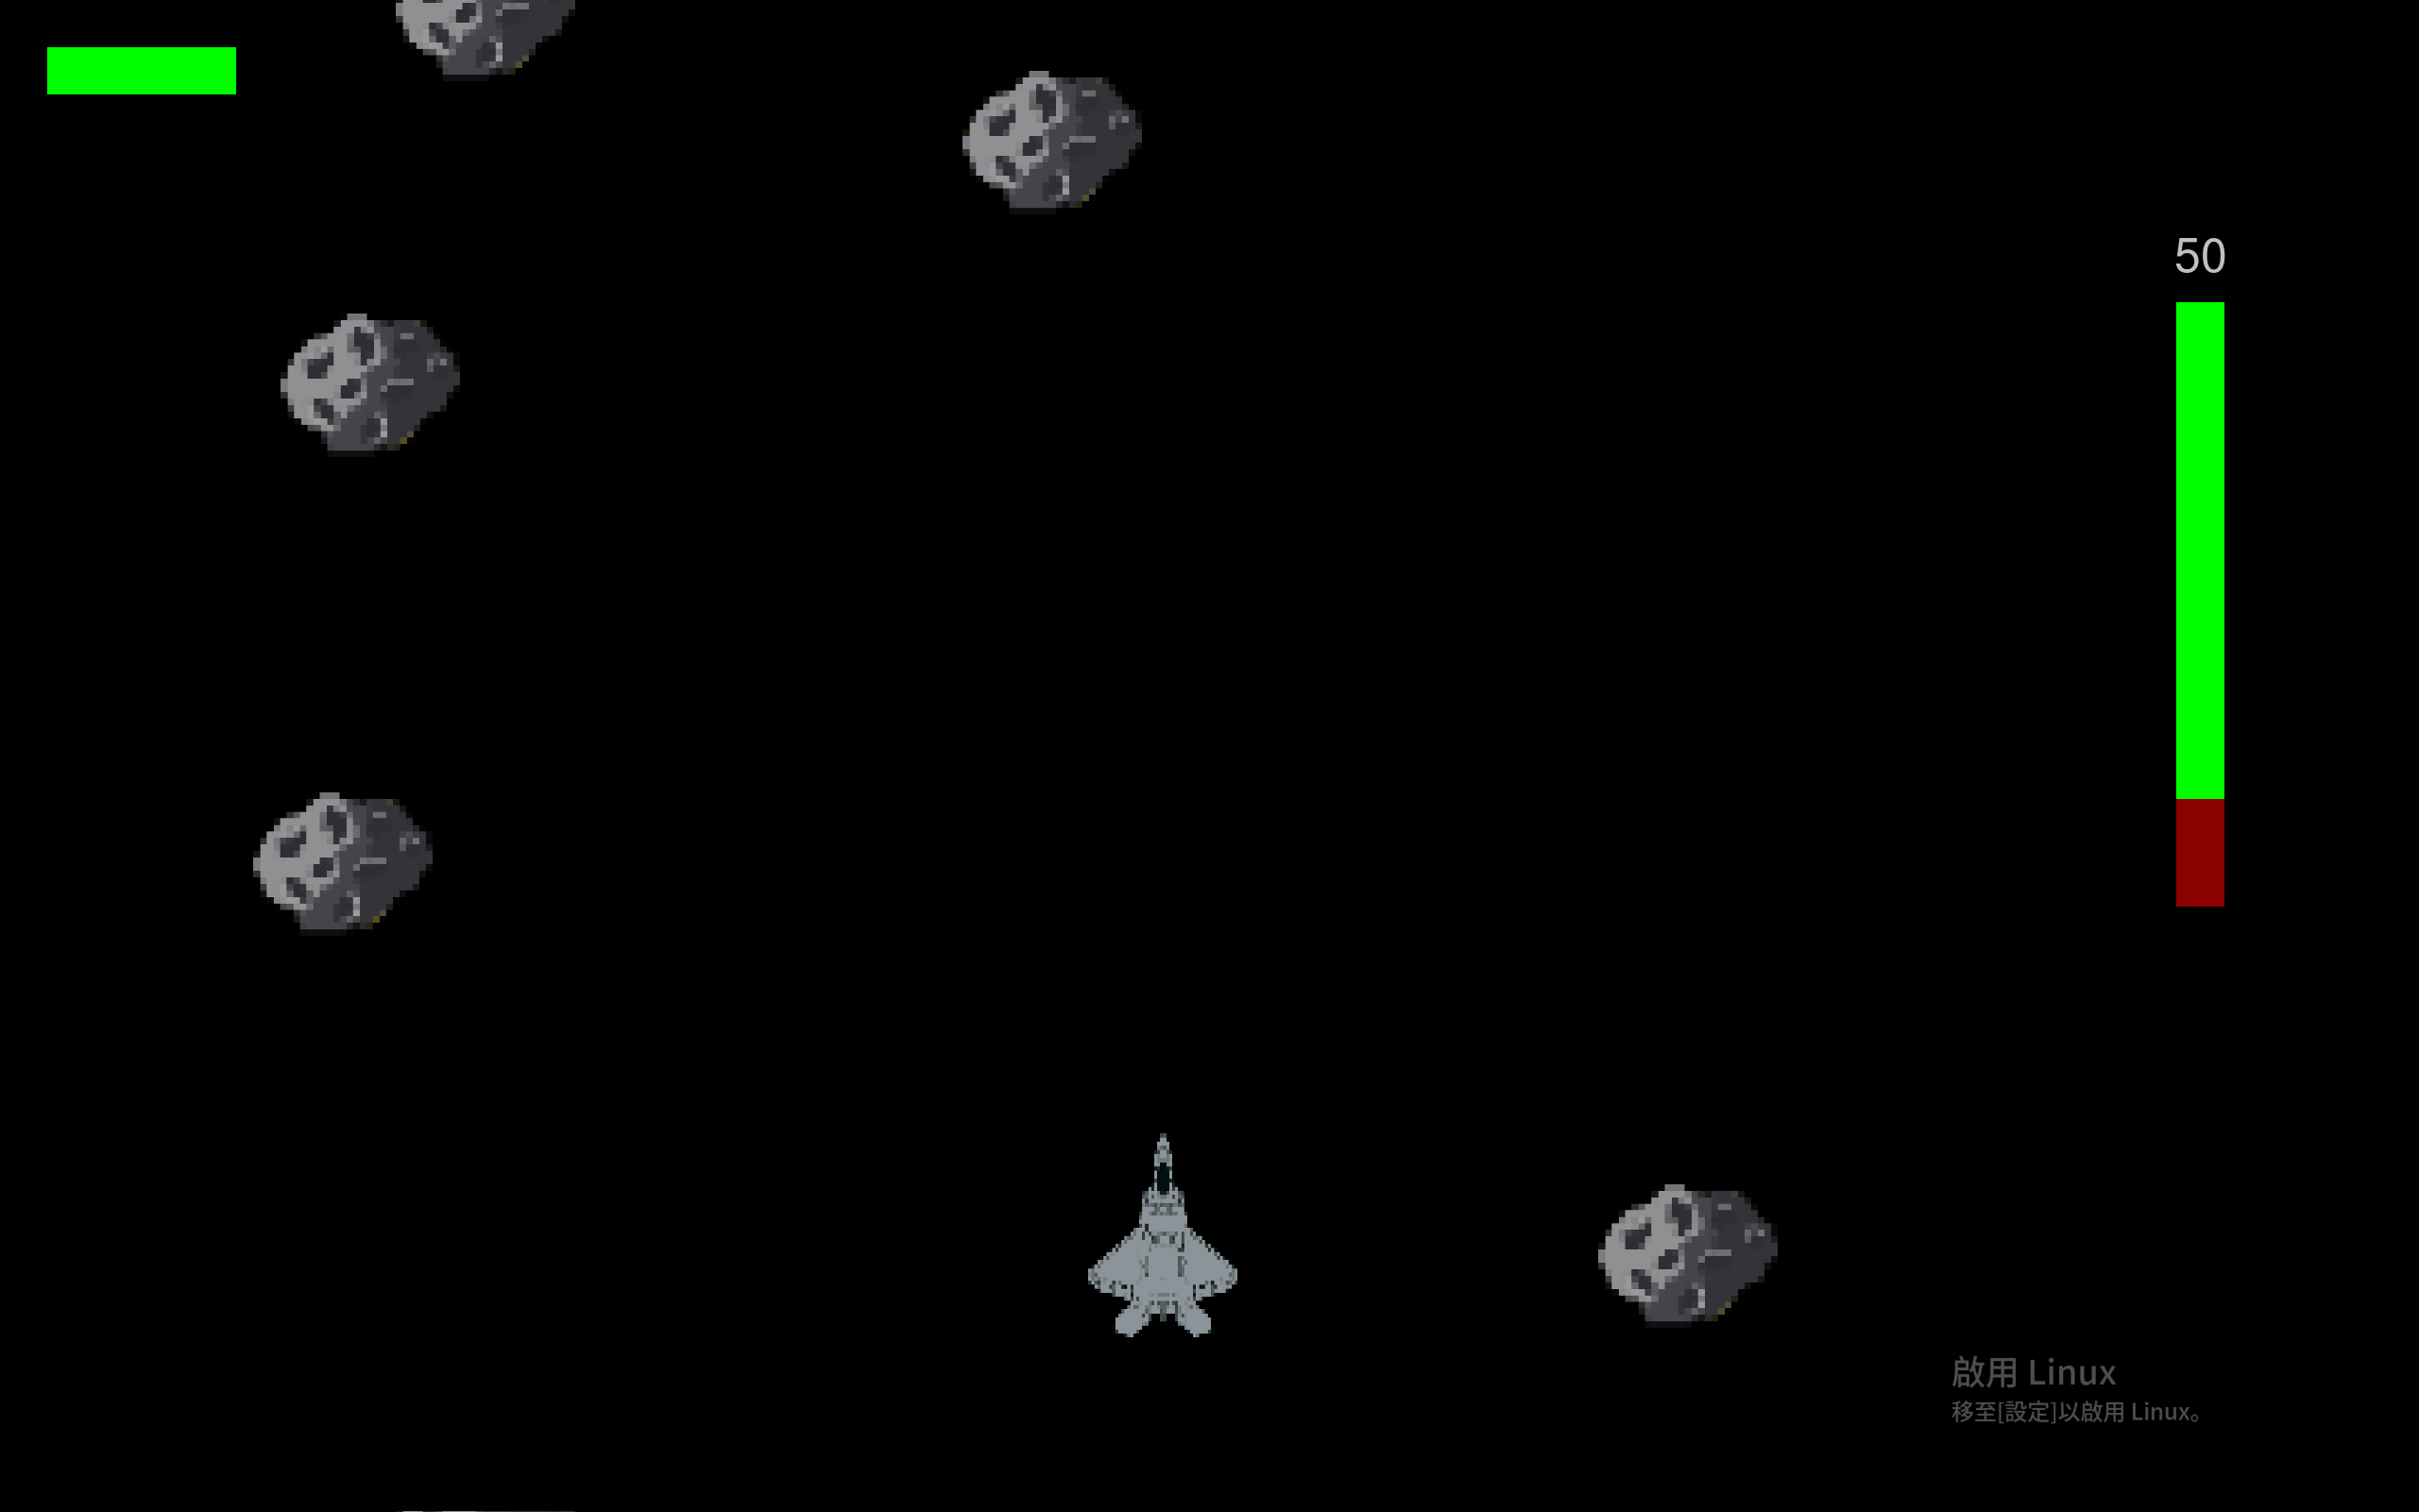
\includegraphics[width=\linewidth]{src/game.png}
\end{boxpar}
\begin{boxpar}{Dandelion}{結尾}
    在這次的自主學習,我發現寫程式一直以來不是一個人的事,是大家的事。自行找答案更是一位程式設計師必須具備的基本能力。所以未來如果我有參與其他活動也會盡力的與組員有良好的溝通並且在麻煩別人之前自己找尋答案以更有效率的完成大家最後的共同目標。
\end{boxpar}
\end{large}
\end{document}
